\documentclass{article}

\usepackage[a4paper, total={6in, 9in}]{geometry}


\usepackage[utf8]{inputenc}
\usepackage{multirow}
\usepackage{amsmath}
\usepackage{amsfonts}
\usepackage{amssymb}

\usepackage{amsthm}
\usepackage{french}

\usepackage{graphicx}

\input{insbox}

\usepackage{hyperref}
\hypersetup{
    colorlinks=true,
    linkcolor=blue,
    filecolor=magenta,      
    urlcolor=cyan,
}

\begin{document}

\begin{titlepage}

\begin{center}
\begin{tabular}{ccc}
\multirow{7}{*}{
\includegraphics[width=0.2\textwidth]{images/Ankatso.png}\hspace{0cm}} & 
\underline{\large{UNIVERSITE D'ANTANANARIVO}} &
\multirow{7}{*}{\hspace{0cm}
\includegraphics[width=0.2\textwidth]{images/Sciences.png}} \\ & & \\ & 
\underline{\large{FACULTE DES SCIENCES}} & \\ & \\ & 
\underline{\large{DEPARTEMENT MATHEMATIQUES}} \\ & & \\ & 
\underline{\large{ET INFORMATIQUE}} \\
\end{tabular}
\end{center}

\vspace{4cm}
	
\begin{center}
\definecolor{darkred}{rgb}{0.8,0,0}
\huge{\textbf{\textcolor{darkred}{Analyse de Données Multidimensionnelles}}}
\LARGE{\textbf{\textcolor{darkred}{Théorie et Pratique}}}
\end{center}

\vspace{3cm}

\begin{flushleft}
Élaboré par: \\
\large{ANDRIAMANANA Hajaniaina Rivo Hery} \\
\large{RAMANANTSOA Zo Samoela Reno} 
\newline

\large{Mathématiques Appliquées} \\
\large{\textit{\underline{Spécialité:}}} Combinatoire et Optimisation
\end{flushleft}
	
\vspace{3cm}
	
\flushright{\underline{Année universitaire}: 2018-2019}

\end{titlepage}

\tableofcontents

\section{Introduction}

Les méthodes d'analyse de données ont commencées a être développées dans les années 50, poussées par le développement de l'informatique et du stockage des données qui depuis n'a cesse de croitre. L'analyse de données a surtout été développée en France par J.P. Benzecri [Ben80a], [Ben80b] qui a su par l'analyse des correspondances représenter les données de manière simple et interprétante.
\newline

Aujourd'hui les méthodes d'analyse de données sont employées dans un grand nombre de domaines qu'il est impossible d'énumérer, a l'instar du marketing pour l'étude des marches ou de l'étude des données météorologiques.
\newline

Les analyses factorielles constituent la plupart des analyses de données. Elles sont fondées sur un principe unique, c'est pour cela que nous pouvons parler de l'analyse factorielle [EP90]. Ce principe repose sur le fait que les deux nuages de points représentant respectivement les lignes et les colonnes du tableau étudié (tableau 1.1) sont construits et représentés sur des graphiques. Ces représentations des lignes et des colonnes fortement liées entre elles permettent une analyse plus aisée pour l'opérateur. Parmi les divers méthodes d'analyse factorielle, on peut citer l'analyse en composantes principales, l'analyse factorielle des correspondances, l'analyse des correspondances multiples et l'analyse factorielle discriminante.
\newline

Dans ce pressent projet, nous nous intéresserons surtout a l'analyse en composantes principales que nous notons par la suite ACP. C'est une des premières analyses factorielles, et certainement aujourd'hui l'une des plus employées. Dans [LMP95], nous trouvons l'historique de cette méthode qui fut conçue par Karl Pearson en 1901. Elle est sans doute a la base de la compréhension actuelle des analyses factorielles.
\newline

Son utilisation a cependant été plus tardive avec l'essor des capacités de calculs. Les principales variantes de l'ACP viennent des différences de transformations du tableau de données. Ainsi, le nuage de points peut être centre ou non, réduit ou non.
Le cas le plus étudié, et que nous présentons ici, est lorsque le nuage de point est centre et réduit ; dans ce cas nous parlons d'ACP normée. D'autres variantes existent telle que l'analyse en composante curviligne [DH97] pour remédier au fait que les projections sont linéaires, ou encore l'analyse en composantes indépendantes pour la séparation de sources [Pha96].

\newpage

\section{Théorie}

\subsection{Tableau de données}

L'\textbf{A}nalyse en \textbf{C}omposante \textbf{P}ricipale s'intéresse à l'étude des tableaux de données rectangulaires dont les lignes sont appelées \textit{Individus} et les colonnes sont appelées \textit{Variables}.
\newline

L'image ci-dessous illustre un tableau de données a \textit{n-individus} et a \textit{p-variables}. Un \textit{individu} est noté $i=(x_{i1},x_{i2}, ... ,x_{ip}) \in \mathbb{R}^p$ et une \textit{variable} est notée $x_j=(x_{1j},x_{2j}, ... ,x_{nj}) \in \mathbb{R}^n$
\newline

\underline{NB:} Il est important de souligner que les \textit{variables} sont \textbf{quantitatives} en ACP, c'est à dire que $x_{ij} \in \mathbb{R}, \; \forall (i,j) \in [n]\times[p].$

\begin{figure}[h!]
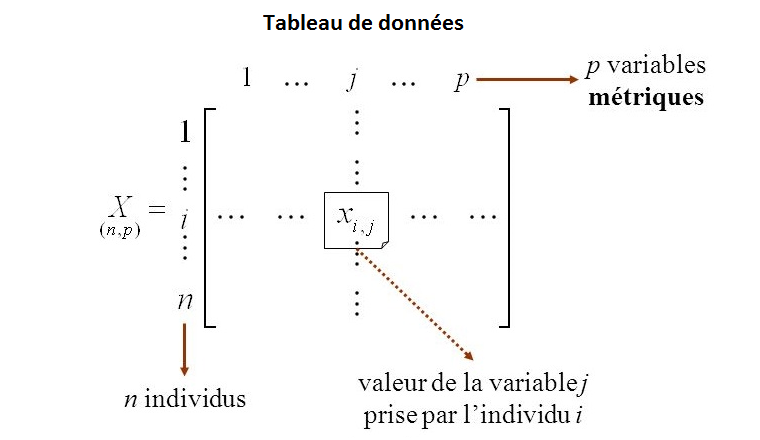
\includegraphics[width=\linewidth]{images/tableau.png}
\end{figure}

\subsection{Moyenne et Variance}

Pour une \textit{variable} ${x_j}$, on note sa moyenne $\bar{x}_j$ et son écart-type $s_j$ telles que:

\begin{equation*}
\bar{x}_j=\frac{1}{n}\sum_{i=1}^{n}{x_{ij}} \;\;\;\;\;\;\;\;\;\; s_j=\sqrt{\frac{1}{n}\sum_{i=1}^{n}{(x_{ij}-\bar{x}_j)^2}}
\end{equation*}

\subsection{Distance et Point moyen}
En ACP, il est important de savoir quels \textit{individus} sont proches les un des autres, pour pouvoir, si possible, créer des groupes d'\textit{individus} selon leur proximité. Il est alors nécessaire de définir une distance entre deux \textit{individus} i et i', soit d cette distance:

\begin{equation*}
d^2(i,i')=\sum_{j=1}^{p}{(x_{ij}-x_{i'j})^2} 
\end{equation*}

\newpage

De plus, à partir de la moyenne de chaque \textit{variables}, on construit un point noté G et appelé \textbf{point moyen} du nuage des \textit{individus}, ce point peut être interprété comme le centre de gravité du nuage des \textit{individus}:

\begin{equation*}
G=(\bar{x}_1,\bar{x}_2,...,\bar{x}_p)
\end{equation*}

\subsection{Centrage et Réduction}
Ayant le point moyen, qui peut être vue comme le centre de gravité du nuage, il est conseillé de translater notre nuage de telle façon que G soit confondue avec le centre du repère, cela ce traduit par: ``Replacer $x_j$ par $x_{ij}-\bar{x}_j$ dans le tableau de données'';
\newline

Cette processus s'appelle \textbf{centrage} et elle améliore grandement l'affichage et l'interprétation des graphiques de nos données.

\begin{equation*}
x_{ij} \leftarrow x_{ij}-\bar{x}_j \;\;\;\;\; \forall i \in [n], \; \forall j \in [p],
\end{equation*}
\newline

Parfois, les \textit{variables} ne sont du même unité, ceci peut entrainer une ambiguïté dans l'interprétation des données, en effet, une variable a une ``quantité'' plus petite, dans le tableau, lorsqu'elle est exprimé en mettre, que lorsqu'elle est exprimé en centimètre. Ce qui peut entrainer, respectivement aux unités, une faible ou une forte importance par rapport aux autres variables qui faussera alors l'analyse.
\newline

Un moyen efficace d'éviter ce problème est la \textbf{réduction}, elle consiste a diviser les \textit{variables} par leur écart-type.
\newline

Comme on a convenu plutôt qu'il est préférable de centrer les \textit{variables}, alors le \textbf{centrage} et la \textbf{réduction} se traduit par: ``Replacer $x_j$ par $(x_{ij}-\bar{x}_j)/s_j$ dans le tableau de données'';

\begin{equation*}
x_{ij} \leftarrow \frac{x_{ij}-\bar{x}_j}{s_j}  \;\;\;\;\; \forall i \in [n], \; \forall j \in [p]
\end{equation*}
\newline

\underline{NB:} Après le centrage et la réduction, nos nouvelles \textit{variables} sont alors ``asymptotiquement'' de moyenne nulle et de variance égale a un. c'est a dire:

\begin{equation*}
\bar{x}_j \approx 0 \;\;\;\;\; s_j^2 \approx 1 \;\;\;\;\; \forall j \in [p]
\end{equation*}

\subsection{Inertie}

Par définition, l'inertie \textit{I} des données est:

\begin{equation*}
I = \frac{1}{n} \sum_{i=1}^n \sum_{j=1}^p {\left( \frac{x_{ij}-\bar{x}_j}{s_j} \right)}^2
\end{equation*}

C'est donc, au coefficient 1/n près, la somme des carrés de toutes les cellules du tableau de données après centrage et réduction, mais elle peut également être interprétée par rapport aux \textit{individus} et aux \textit{variables}.

\newpage

\begin{flushleft}
\textbf{Inertie et Individus}
\end{flushleft}

Soit l'individu $i \in [n]$, la quantité $\sum_{j=1}^p {\left( \frac{x_{ij}-\bar{x}_j}{s_j} \right)}^2$ de l'inertie represente la distance au carrée entre cet individu et le point moyen G. Par conséquent, l’inertie peut être vue comme la somme des carres des distances au centre de gravite pour tous les individus.
\newline

Ainsi, l’inertie renseigne sur la ``forme'' du nuage des individus. En effet, plus la distance entre les individus sont grande (resp. petite), plus l'inertie est grande (resp. petite).

\begin{flushleft}
\textbf{Inertie et Variables}
\end{flushleft}

Dans la définition de l'inertie, les deux somme $\sum$ peuvent être interverti, ainsi, on a une autre expression:

\begin{equation*}
I = \frac{1}{n} \sum_{j=1}^p \sum_{i=1}^n {\left( \frac{x_{ij}-\bar{x}_j}{s_j} \right)}^2
\end{equation*}

Ici, on peut remarquer que la quantité $\sum_{i=1}^n {\left( \frac{x_{ij}-\bar{x}_j}{s_j} \right)}^2$ correspond au carré de la norme de la variable centrée réduite $x_j$ ou $j \in [p]$. Or cette quantité est égale à n, ainsi, l'inertie est toujours égale au nombre de variables, en effet:

\begin{align*}
I &= \frac{1}{n} \sum_{j=1}^p \sum_{i=1}^n {\left( \frac{x_{ij}-\bar{x}_j}{s_j} \right)}^2 \\
  &= \frac{1}{n} \sum_{j=1}^p \left( \frac{1}{s_j^2} \; n{s_j^2} \right) \\  
  &= \frac{1}{n} \sum_{j=1}^p \left( \frac{1}{s_j^2} \; n{s_j^2} \right) \\
  &= \frac{1}{n} \sum_{j=1}^p n \\
  &= \frac{1}{n} \; pn \\
  &= p
\end{align*}
\\

\subsection{Représentation Simplifiée}

On a vu que les \textit{variables} sont des vecteurs de $\mathbb{R}^p$, alors, quand $p > 3$, il n'est plus possible de représenter les variables. L'ACP vise a fournir une image simplifiée du nuage des \textit{individus} la plus fidèle possible, c'est a dire, trouver une sous-espace de dimension plus petite qui résume au mieux les données.
\newline

\newpage

\begin{flushleft}
\textbf{Comment retrouver la meilleur sous-espace?}
\end{flushleft}

Pensons pour cela a l’image d’un chameau, la figure ci-dessous propose deux représentations simplifiées de cette image: des représentations en dimension 2, la vue de face et la vue de profil.

\begin{figure}[h!]
\centering
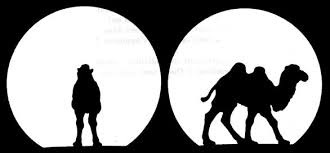
\includegraphics[width=200px]{images/chameau.png}
\end{figure}

Il est évident de dire que la meilleure représentation simplifiée est la vue de profil. La raison est que l’image projetée du chameau dans ce plan est plus proche de l’image initiale dans le sens ou la variabilité des points qui la représentent est plus grande et donc restitue mieux la variabilité des points d’origine en dimension 3.
\newline

On a alors les étapes suivantes pour retrouver analytiquement la meilleure représentation simplifiée du nuage des \textit{individus}:

\begin{flushleft}
Étape 1: \textbf{Trouver l'axe qui déforme le moins possible le nuage}
\end{flushleft}

On cherche un axe dans $\mathbb{R}^p$ de sorte que les distances entre les points initiaux i (\textit{individu}) soient les plus proches possibles de leurs projetés orthogonaux sur cette axe et cela en tenant compte de tous les autres points. Notons $\vec{u}_1$ la direction de cet axe, et $H_i$ la projetée orthogonale de i.
\newline

\InsertBoxL{0}{\quad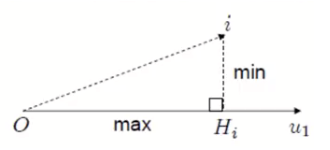
\includegraphics[width=200px]{images/projection.png}\quad} %

Le but est de minimiser la distance $iH_i$, ce qui revient a maximiser la distance $OH_i$
\newline

Plus formellement, on cherche la direction $\vec{u}_1$ de $\mathbb{R}^p$ telle que $\sum_{i=1}^n OH_i^2$ soit maximum.
\newline

On dira qu’on cherche $\vec{u}_1$ telle que l’inertie projetée $I_p$ est maximum.

\begin{flushleft}
Étape 2: \textbf{Trouver le meilleur plan}
\end{flushleft}

Cette fois ci, on cherche le meilleur plan $\mathcal{P}$ ou l'inertie projetée $I_p$ est maximale sur ce plan, pour ce faire, on cherche une direction $\vec{u}_1$ qui maximise $I_p$ (fait à l'étape 1), puis on cherche une autre direction $\vec{u}_2$ orthogonale a $\vec{u}_1$ et qui, elle aussi, maximise $I_p$.
\newline

Le plan meilleur plan $\mathcal{P}$ est formé par les deux meilleurs axes de directions respectives $\vec{u}_1$ et $\vec{u}_2$, orthogonales l'un a l'autre.

\begin{flushleft}
Étape 3: \textbf{Trouver un troisième meilleur axe}
\end{flushleft}

On peut chercher un troisième axe et essentiellement, chercher les axes les un après les autres et a chaque fois, un axe doit être orthogonal aux axes précédents, et maximise l'inertie projetée $I_p$.
\newline

\begin{flushleft}
\underline{NB}: A l'issu de ces étapes, on appel les axes de direction $\vec{u}_j,j \in [p]$, \textbf{Composantes Principales}
\end{flushleft}

\newpage

\section{Pratique de l'ACP}

\subsection{Données}

Nous allons étudier les résultats des épreuves de Decastar et des Jeux Olympiques, dont les \textit{Individus} sont les joueurs et les \textit{Variables} sont les jeux eux même, soient:
\newline
\\
- 100m, pour la course de vitesse 100m \\
- Longueur, pour le saut en longueur \\
- Poids, pour le lancé de poids \\
- Hauteur, pour le saut en hauteur \\
- 400m, pour la course de 400m \\
- 110m H, pour la course de vitesse 110m Homme \\
- Disque, pour le lancé de disque \\
- Perche, pour le lancé de perche \\
- Javelot, pour le lancé de javelot \\
- 1500m, pour la course d'endurance 1500m \\
- Classement, pour la classement finale de chaque joueur \\
- Points, pour le point finale obtenu par chaque joueur \\
- Competition, pour le type de compétition \\

Voici une partie des données utilisées:

\begin{figure}[h!]
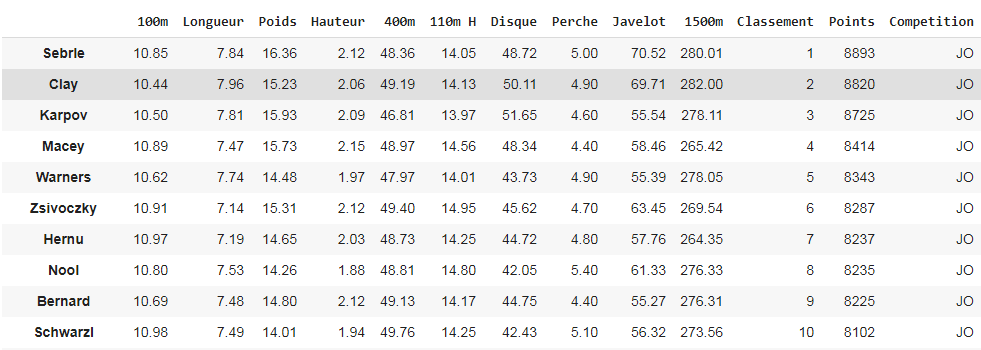
\includegraphics[width=\linewidth]{images/data_initials.png}
\end{figure}

\subsection{Centrage et Reduction}

On voit bien que les \textit{variables} ne sont pas de même unité, alors en plus du centrage, on va aussi réduire les variables. Après avoir fait cette étape dans un logiciel statistique. On veut confirmer que les \textit{variables} sont bien centrées et réduites, c'est a dire qu'elles sont asymptotiquement de moyenne nulle et de variance égale a un. Ainsi on a la figure ci-dessous:

\begin{figure}[h!]
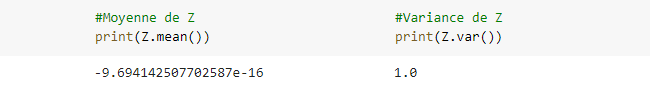
\includegraphics[width=\linewidth]{images/mean_variance.png}
\end{figure}

D'après ces résultats, les moyennes et les variances de nos \textit{variables normalisées} tendent bien vers 0 et 1 respectivement.
\newline

\newpage

\begin{flushleft}
\underline{NB}: A partir d'ici, on va travailler avec les \textbf{Données Normalisées} 
\end{flushleft}

\subsection{Les axes a retenir}

Un moyen de trouver les \textbf{composantes principales} ou \textbf{meilleurs axes} est de calculer les \textit{valeurs propres} de la matrice de covariances des \textit{variables}. En ordonnant ces \textit{valeurs propres} par ordre décroissant, les \textit{vecteurs propres} associes deviennent les directions $\vec{u}_j,j \in [p]$ des \textbf{composantes principales}.
\newline

La quantité d'informations portée par un axe est alors proportionnelle a la \textit{valeur propre} associée, ainsi, un nombre $k<p \in \mathbb{N}^*$ d'axes suffit pour représenter les individus. En effet, il y a des axes dans leur \textit{valeur propre} est neglisable par rapport a celles des autres.
\newline

Il y a plusieurs méthodes pour retrouver les axes à éliminer, mais pour notre problème, on va utiliser la méthode du coudé, d'après \href{https://fr.qaz.wiki/wiki/Elbow_method_(clustering)}{Wikipedia - Méthode du coude (clustering)} 
\newline

\textit{La méthode du coude est une heuristique utilisée pour déterminer le nombre de clusters (axes dans notre cas) dans un ensemble de données. La méthode consiste à tracer la \textbf{variation expliquée} en fonction du nombre de clusters, et à choisir le coude de la courbe comme le nombre de clusters à utiliser. La même méthode peut être utilisée pour choisir le nombre de paramètres dans d'autres modèles basés sur les données, comme le nombre de composants principaux pour décrire un ensemble de données}
\newline

Pour ce faire, on a donc besoin des variation expliquée, qui sont les \textit{valeurs propres} associées à nos axes et de trace la courbe de la fonction f définie par:

\begin{equation*}
f(V_e)=\frac{(n-1)}{n}*V_e \quad , \; V_e \; est \; la  \; variance \; explicative.
\end{equation*}

\begin{figure}[h!]
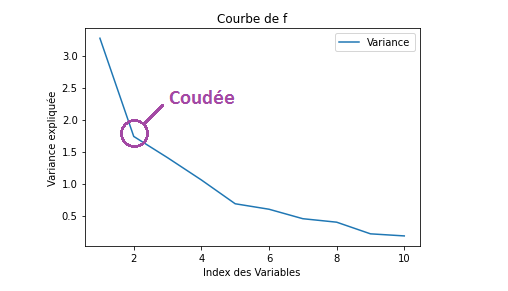
\includegraphics[width=\linewidth]{images/courbe_ve.png}
\end{figure}

D'après la graphe de la fonction - variance expliquée - on ne va donc retenir que les deux premières \textbf{composantes principales} suivant l'ordre décroissante des \textit{valeurs propres}.

\newpage

On peut ainsi positionner les individus dans le plan formé par ces deux \textbf{composantes principales}. On a alors la figure suivante:

\begin{figure}[h!]
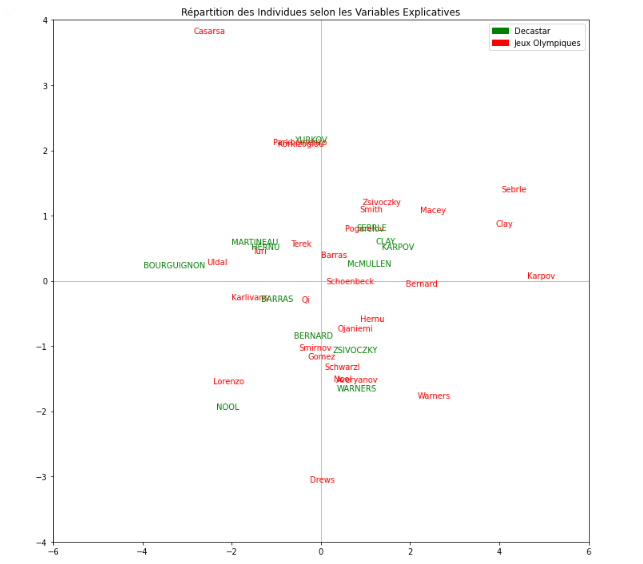
\includegraphics[width=\linewidth]{images/graph-plan.png}
\end{figure}

\begin{flushleft}
\textbf{Interprétation du premier axe (Horizontale)}
\end{flushleft}

On peut remarquer du premier axe qu'il départage les joueurs ayant un bon classement a ceux qui ont un mauvais classement pendant les deux compétitions.
En effet, les joueurs \textbf{Karpov} et \textbf{Clay} qui sont le deuxieme et le troisième dans le classement des Jeux Olympiques, et des Jeux de Decastar sont placés à droite dans la premier axe, alors que le joueur \textbf{Uldal}, avant dernier du classement des JO et le joueur \textbf{Bourguignon}, dernier du classement de Decastar sont placés a gauche dans la premier axe. 

\begin{flushleft}
\textbf{Interprétation du deuxième axe (Verticale)}
\end{flushleft}

On peut remarquer du deuxième axe qu'il départage les joueurs forts dans les épreuves de vitesse et d'endurance a ceux qui sont fort dans les épreuves de lancés (poids, perche, javelot).
En effet, les joueurs \textbf{Carcasa} et \textbf{Yurkov} qui sont meilleurs dans les épreuves de lancées respectivement aux JO et Decastar sont placées en haut du deuxième axe, alors que les joueurs \textbf{Drews} et \textbf{Bernard} forts aux épreuves respectives d'endurances pendant les JO et de vitesse pendant le Decastar sont placés en bas du deuxième axe.

\newpage

Le cercle de corrélation ci-dessous peut nous donner encore plus d'informations sur nos données par l'interprétation des variables.

\begin{figure}[h!]
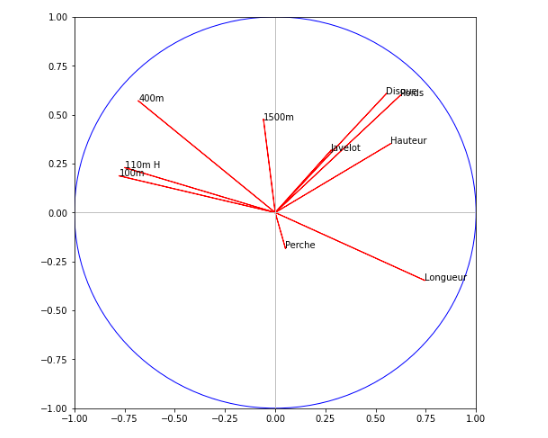
\includegraphics[width=\linewidth]{images/cercle_cor.png}
\end{figure}

\begin{flushleft}
\textbf{Interprétation des corrélations positives}
\end{flushleft}

\begin{itemize}
\item On remarque que les épreuves \textbf{100m} et \textbf{110m H} sont très corrélées positivement, c'est a dire que les joueurs forts sur l'une sont aussi forts sur l'autre. Ce sont les joueurs fort en vitesse qu'on a vu dans l'interprétation des \textbf{composantes principales}.
\item De même, les épreuves \textbf{Poids}, \textbf{Disque} et \textbf{Javelot} sont corrélées positivement, cette corrélation regroupe les épreuves de lancés. Ceci aussi renforce notre interprétation des \textbf{composantes principales}.
\end{itemize}

\begin{flushleft}
\textbf{Interprétation des corrélations négatives}
\end{flushleft}

\begin{itemize}
\item On remarque que les épreuves \textbf{400m} et \textbf{Longueur} sont très corrélées négativement, c'est a dire que les joueurs meilleurs sur l'un sont mauvais sur l'autre. On peut remarquer dans ce cas le joueur \textbf{Martineau} pendant le Decastar, ou il est très fort en \textbf{400m} mais très mauvais en \textbf{Longueur}, ou le joueur \textbf{Karpov} pendant les JO, qui est très faible en \textbf{400m} mais très fort en \textbf{Longueur}.
\end{itemize}

\newpage

\section{Pratique de l'AFC}
\subsection{Recherche des axes a retenir et des coordonnées des points lignes et des points colonnes}

Nous pouvons voir sur le tableau ci-dessous une partie des données de la répartition des nombres de médaillés sur les épreuves des Jeux Olympiques par les différents pays participants:

\begin{figure}[h!]
\centering
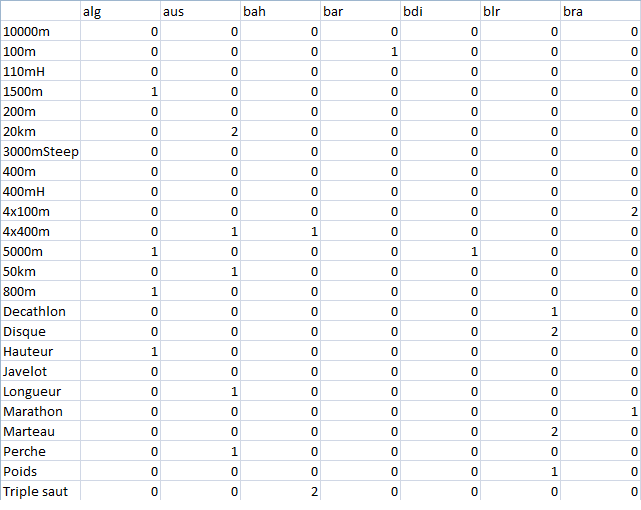
\includegraphics[scale=0.75]{images/Extrait.PNG}
\caption{Extrait de la repartition des nombres de medailles}
\end{figure}

Après avoir centre puis réduit le tableau de données, nous calculons les valeurs propres de la matrice d'inertie associée.

\begin{figure}[h!]
\centering
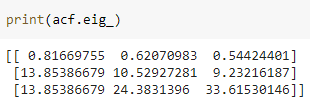
\includegraphics[scale=0.75]{images/VP.PNG}
\caption{Valeurs Propres de la matrice associée}
\end{figure}

\newpage

L'étude des valeurs propres permet ensuite de déterminer les axes a retenir.

\begin{figure}[h!]
\centering
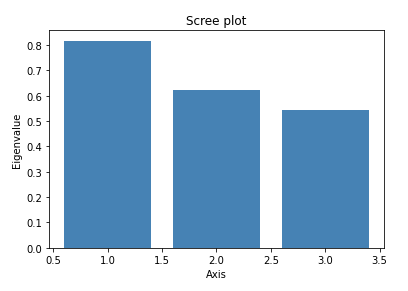
\includegraphics[scale=0.75]{images/Plot_VP.PNG}
\caption{Représentation des Valeurs Propres en pourcentage de la variance}
\end{figure}

\begin{figure}[h!]
\centering
\includegraphics[scale=0.75]{images/VP_cumule.PNG}
\caption{Représentation des Valeur Propres en pourcentage cumule de la variance}
\end{figure}

Nous retiendrons alors les 3 axes associes a ces valeurs propres pour l'AFC: en effet ces 3 axes permettent d'expliquer environ 35\% de la variance totale des données. Nous déterminons ensuite les coordonnées, les contributions et les $\cos^2$ de chacun des points lignes et points colonnes pour tous les axes factoriels.
\newline

On procède au mapping simultané des points lignes et des points colonnes: nous représentons dans le même repère des axes retenus les points lignes et les points colonnes afin d'en dégager l'interprétation des données.

\newpage

Dans notre cas, nous effectuons le mapping sur l'axe 1 et 2:

\begin{figure}[h!]
\centering
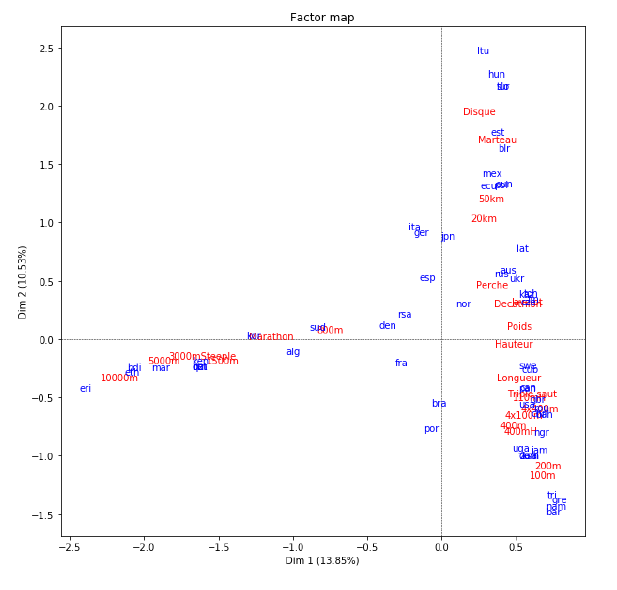
\includegraphics[scale=0.8]{images/Mapping.PNG}
\caption{Mapping sur l'axe 1 et 2 des points lignes et des points colonnes}
\end{figure}

\subsection{Interpretation}

Dans notre interprétation, nous allons nous baser sur le mapping effectue sur les axes 1 et 2 précédent.
\newline

En reliant chaque point ligne et chaque point colonne a l'origine, on peut associer a chaque point un vecteur relatif a ce point. Ainsi, en étudiant les produits scalaires entre chaque vecteur nous distinguons essentiellement 3 cas: soit le produit scalaire est positif, soit il est négatif, soit il est proche de zero.
\newline

Dans le cas d'un produit scalaire positif, nous avons une conjonction entre les vecteurs: on a une forte correspondance entre les vecteurs.
\newline

Si le produit scalaire est négatif, nous avons une opposition entre les vecteurs: on a une forte incompatibilité entre les vecteurs.
\newline

Enfin lorsque le produit scalaire est nul, nous avons une quadrature entre les vecteurs: il n'y a pas de corrélation entre les vecteurs.
\newline

Ainsi, nous remarquons que le plan est divise en 3 régions de conjonctions.
\newline

Premièrement, nous remarquons une région ou se concentrent principalement les épreuves de forces tels que le lance de poids, le lance de disque, le lance de marteau,... ou dominent principalement domines par les Européens (Biélorussie, Russie,...).
\newline

Deuxièmement, nous observons une région ou l'on retrouve surtout les épreuves de course d'endurance telles que le 10000m, le 5000m, le marathon,... ou dominent principalement les Africains (Kenya, Éthiopie,...).
\newline

Puis finalement, nous avons une dernière région ou se concentrent surtout les épreuves de courses de vitesse telles que le 100m, le 200m, le 4*100m,... ou dominent principalement les Américains (USA, Jamaïque,...).
\newline

Ensuite, nous remarquons que la région ou se concentrent les épreuves de forces est en opposition avec celle ou se concentrent les épreuves de vitesses. Nous en déduisons que les athlètes doués en épreuves de forces sont généralement moins bons pour les épreuves de vitesses et inversement. Par conséquent, les pays ayant reçus plus de médailles dans les épreuves de forces ont généralement eu moins de médailles dans les épreuves de vitesses et réciproquement. Ainsi les Européens sont généralement bons en épreuve de force tel que le lance de marteau ou le lance de disque mais sont mauvais au 100m ou 200m. Tandis que les Américains sont plutôt bon au 100m et 200m, mais mauvais aux épreuves de lances(disques, marteau,...).
\newline

Enfin, nous remarquons que la région ou se concentrent les épreuves d'endurance est en quadrature avec ces deux régions. Donc les athlètes qui sont bons au épreuves d'endurance sont généralement moyens aux épreuves de forces et aux de vitesses. Par conséquent, les pays ayant remportes plusieurs médailles dans ces disciplines ne sont ni avantages ni désavantages dans les deux autres sortes d'épreuves. Ainsi les Africains qui sont généralement bons au marathon ne sont ni excellent ni mauvais ni au 100m ni au lance de marteau.

\end{document}
